%%%%%%%%%%%%%%%%%%%%%%%%%%%%%%%%%%%%%%%%%%%%%%%%%%%%%%%%%%%%%%%%%%%%%
%%%
%%% Set these variables appropriately
%%%
\newcommand{\AUTHORS}{Marcela Melara, Annie Edmundson, Ohad Fried}
\newcommand{\TITLE}{Multisurf: MITM detection using multiple HTTP clients}
\newcommand{\KEYWORDS}{}
\newcommand{\CONFERENCE}{}
\newcommand{\PAGENUMBERS}{yes}       % "yes" or "no"
\newcommand{\TOAPPEAR}{no}
%%%
%%%
%%%%%%%%%%%%%%%%%%%%%%%%%%%%%%%%%%%%%%%%%%%%%%%%%%%%%%%%%%%%%%%%%%%%%

%%%% Setup the document/page
\documentclass[pdftex,twoside,twocolumn,10pt,letterpaper]{article}
\usepackage{ifthen}

\ifthenelse{\equal{\PAGENUMBERS}{yes}}{%
\usepackage[nohead,
            left=1in,right=1in,top=1in,
            footskip=0.5in,bottom=0.75in     % Room for page numbers
            ]{geometry}
}{%
\usepackage[noheadfoot,columnsep=0.2in,
            margin=1in,centering,truedimen]{geometry}
}

\usepackage{fancyhdr}
\usepackage[numbers,sort]{natbib}
\usepackage{xspace}
\usepackage{booktabs}
\usepackage{subfigure}
\usepackage[T1]{fontenc}
\usepackage{textcomp}
\usepackage{mathptmx}   % Times + Times-like math symbols
\usepackage{courier}
\usepackage[scaled=0.92]{helvet}
\usepackage{url}
\usepackage{color}
\usepackage[pdftex]{graphicx}
\ifthenelse{\isundefined{\wantBW}}{%
  \usepackage[colorlinks]{hyperref}%        % for online version
}{%
  \usepackage[pdfborder={0 0 0}]{hyperref}% % for paper (B&W) version
}
\newcommand{\URL}[1]{\url{#1}}

%%%%% Setup for PDF
\hypersetup{%
pdfauthor = {\AUTHORS},
pdftitle = {\TITLE},
pdfsubject = {\CONFERENCE},
pdfkeywords = {\KEYWORDS},
bookmarksopen = {true}
}

%\setlength{\parindent}{0pt}
%\setlength{\parskip}{0pt}
\renewcommand{\headrulewidth}{0pt}
\newcommand{\Paragraph}[1]{\vspace{-2ex}\paragraph{#1.}}
\setlength{\topmargin}{-.15in}

\ifthenelse{\equal{\PAGENUMBERS}{yes}}{%
  \pagestyle{plain}
}{%
  \pagestyle{empty}
}

\makeatletter\long\def\@makecaption#1#2{
   \vskip 10pt
   \setbox\@tempboxa\hbox{\textsf{#1: #2}}
   \ifdim \wd\@tempboxa >\hsize % IF longer than one line:
       \textsf{#1: #2}\par      % THEN set as ordinary paragraph.
     \else                      % ELSE  center.
       \hbox to\hsize{\hfil\box\@tempboxa\hfil}
   \fi}
\makeatother

\clubpenalty=10000  % Don't allow orphans
\widowpenalty=10000 % Don't allow widows

\title{\textbf{\TITLE}}
\author{\AUTHORS}
\date{}

% Compact itemize and enumerate.  Note that they use the same counters and
% symbols as the usual itemize and enumerate environments.
\def\compactify{\itemsep=0pt \topsep=0pt \partopsep=0pt \parsep=0pt}
\let\latexusecounter=\usecounter
\newenvironment{CompactItemize}
  {\def\usecounter{\compactify\latexusecounter}
   \begin{itemize}}
  {\end{itemize}\let\usecounter=\latexusecounter}
\newenvironment{CompactEnumerate}
  {\def\usecounter{\compactify\latexusecounter}
   \begin{enumerate}}
  {\end{enumerate}\let\usecounter=\latexusecounter}

\newcommand{\comment}[1]{\textcolor{red}{#1}}
\newcommand{\ignore}[1]{}

\newcommand{\xc}[1]{\mbox{\textit{#1}}}
\newcommand{\la}{\leftarrow}
\newcommand{\ra}{\rightarrow}
\newcommand{\somespace}{\hspace{0.1cm}}

\def\discretionaryslash{\discretionary{/}{}{/}}
\def\discretionarydot{\discretionary{.}{}{.}}
\def\discretionarycolon{\discretionary{:}{}{:}}
{\catcode`\/\active
\catcode`\.\active
\catcode`\:\active
\gdef\URLprepare{\catcode`\/\active\let/\discretionaryslash
                 \catcode`\.\active\let.\discretionarydot
                 \catcode`\:\active\let:\discretionarycolon
        \def~{\char`\~}}}%
\def\URL{\bgroup\URLprepare\realURL}%
\def\realURL#1{\tt #1\egroup}%

\newcommand{\eg}{{\em e.g.}, }
\newcommand{\ie}{{\em i.e.}, }
\newcommand{\etal}{{\em et al.\ }}

\def\check{\stackrel{{\scriptscriptstyle ?}}{=}}

\begin{document}
\maketitle

\section{Introduction}
\label{sec:intro}

An increasing number of popular websites support the SSL/TLS protocol, the current standard for encrypting web traffic.
Most commonly seen as part of the HTTPS protocol, SSL/TLS provides data and message confidentiality to protect users browsing the web from malicious attackers attempting to eavesdrop or tamper with traffic. 
Nonetheless, about 48\% of popular websites remain insecure by only supporting HTTP connections~\cite{sslpulse}, which are vulnerable to man-in-the-middle (MITM) attacks.
Because HTTP traffic is not encrypted nor authenticated, an unsuspecting user may be visiting a specific website without realizing that an adversary has modified the contents of these web pages while in transit.

Indeed, such in-flight web page modifications occur in practice with a surprising frequency for various reasons, often resulting in undesirable effects such as injected advertisements, broken pages, and exploitable security vulnerabilities~\cite{tripwires}. 
While the vast majority of changes to web pages in transit have economic incentives for website publishers,~\cite{tripwires} also found that a portion of their measured in-flight modifications was due to injected malware.
To provide web servers with a practical, more affordable alternative to HTTPS, Reis \emph{et al.}~\cite{tripwires} proposed \emph{web tripwires}, client-side scripts that can detect most modifications to unencrypted web pages.

However, this solution requires that website publishers modify their pages to contain these scripts, and users unaware of the installed web tripwires may disregard warning messages as spam.
Furthermore, helping website publishers understand and react to any changes made \emph{en route} does not necessarily help users protect themselves from injected malware.
This paper presents \emph{Multisurf}, a browser extension which checks the integrity of unencrypted web pages helping users detect when their HTTP traffic has been hijacked, and without requiring support from the administrator or owner of the affected website. 
Multisurf's collaborative integrity checks detect in-flight changes to websites through a system of trusted peers, end-hosts run by persons or institutions that a user running the Multisurf client trusts. 
By gathering the peers' versions of requested web content, the client can verify whether the visited web page was tampered with in transit.
Because many changes to web pages \emph{en route} are not of malicious nature, the Multisurf client displays the result of the integrity check and gives the user the option of viewing the peers' versions to help her determine if she accepts the in-flight modifications or if she considers the modifications to be malicious, blacklisting the site. 
Thus, Multisurf leverages out-of-band communication, inter-personal trust and takes user preferences into account giving control to the end user in whether she would like to surf the web in a more aware way.

This paper is organized as follows. In Section \ref{sec:model} we outline our system model. Section \ref{sec:design} details Multisurf's system design and the collaborative integrity check protocol; we evaluate the efficacy and accuracy of Multisurf in Section \ref{sec:eval}. Section \ref{sec:related} describes some related work, and we discuss directions for future work in Section \ref{sec:future}. We conclude in Section \ref{sec:conclusion}.

\section{System Model}
\label{sec:model}

Upon a request for a web page, the Multisurf client engages a user-defined set of trusted peers, trusted end-hosts which mirror the browser's web requests on demand and return the served web content to the client.
Should the client detect any discrepancies between its version of a website and 

Threat Model:
The attacker can only control a client’s access link, and is distant enough from the server’s link to not control all server-to-client traffic. We assume the client is the target (for example, attacker uses an unsecure WiFi network which he shares with client).
An attack in which the adversary has compromised the server’s link is out of the scope of this work.
\section{Design}
\label{sec:design}

The Multisurf system has three main components:
\begin{itemize}
\item The browser extension which interacts with the user.
\item The native client application which is responsible for communicating with the peers and for performing the integrity checks.
\item The peer application which mirrors any requests from the Multisurf client.
\end{itemize}

The browser extension gathers HTTP request and response data while the user browses the web normally.
In the background, the Multisurf extension passes this information to the native client, which solicits all received HTTP requests via SSL to one or more trusted peers.
These also issue the same request for a web page to the web server.
The peer returns its version of the server’s served content to the client.
Figure \ref{fig:protocol} details the client-peer protocol.

To perform the integrity check, the Multisurf client compares the original server web page content with the peers' versions of the request web page.
We have designed various comparison vectors which the client can employ to verify the integrity of the received content for the request web page:
\begin{itemize}
\item A line-by-line comparison of the content. This is a rather coarse-grained comparison metric.
\item The number of script tags in the content. Any discrepancies in this could indicate a malicious script injection.
\item The links contained within \texttt{<script>} tags and \texttt{<a>} tags. This algorithm finds matching elements in the web content being compared. Differing links in the same element may indicate a malicious in-flight injection.
\end{itemize}

The client sends the result of the consistency check back to the browser extension, which displays the results to the user.
In the case of an unsafe website, the browser extension allows the user to view the differing web pages to help her determine if she deems the differences malicious or not.
Should the user decide that an unsafe website is malicous, the extension allows her to blacklist the site for future browsing sessions.

\begin{figure}[h]
\centering
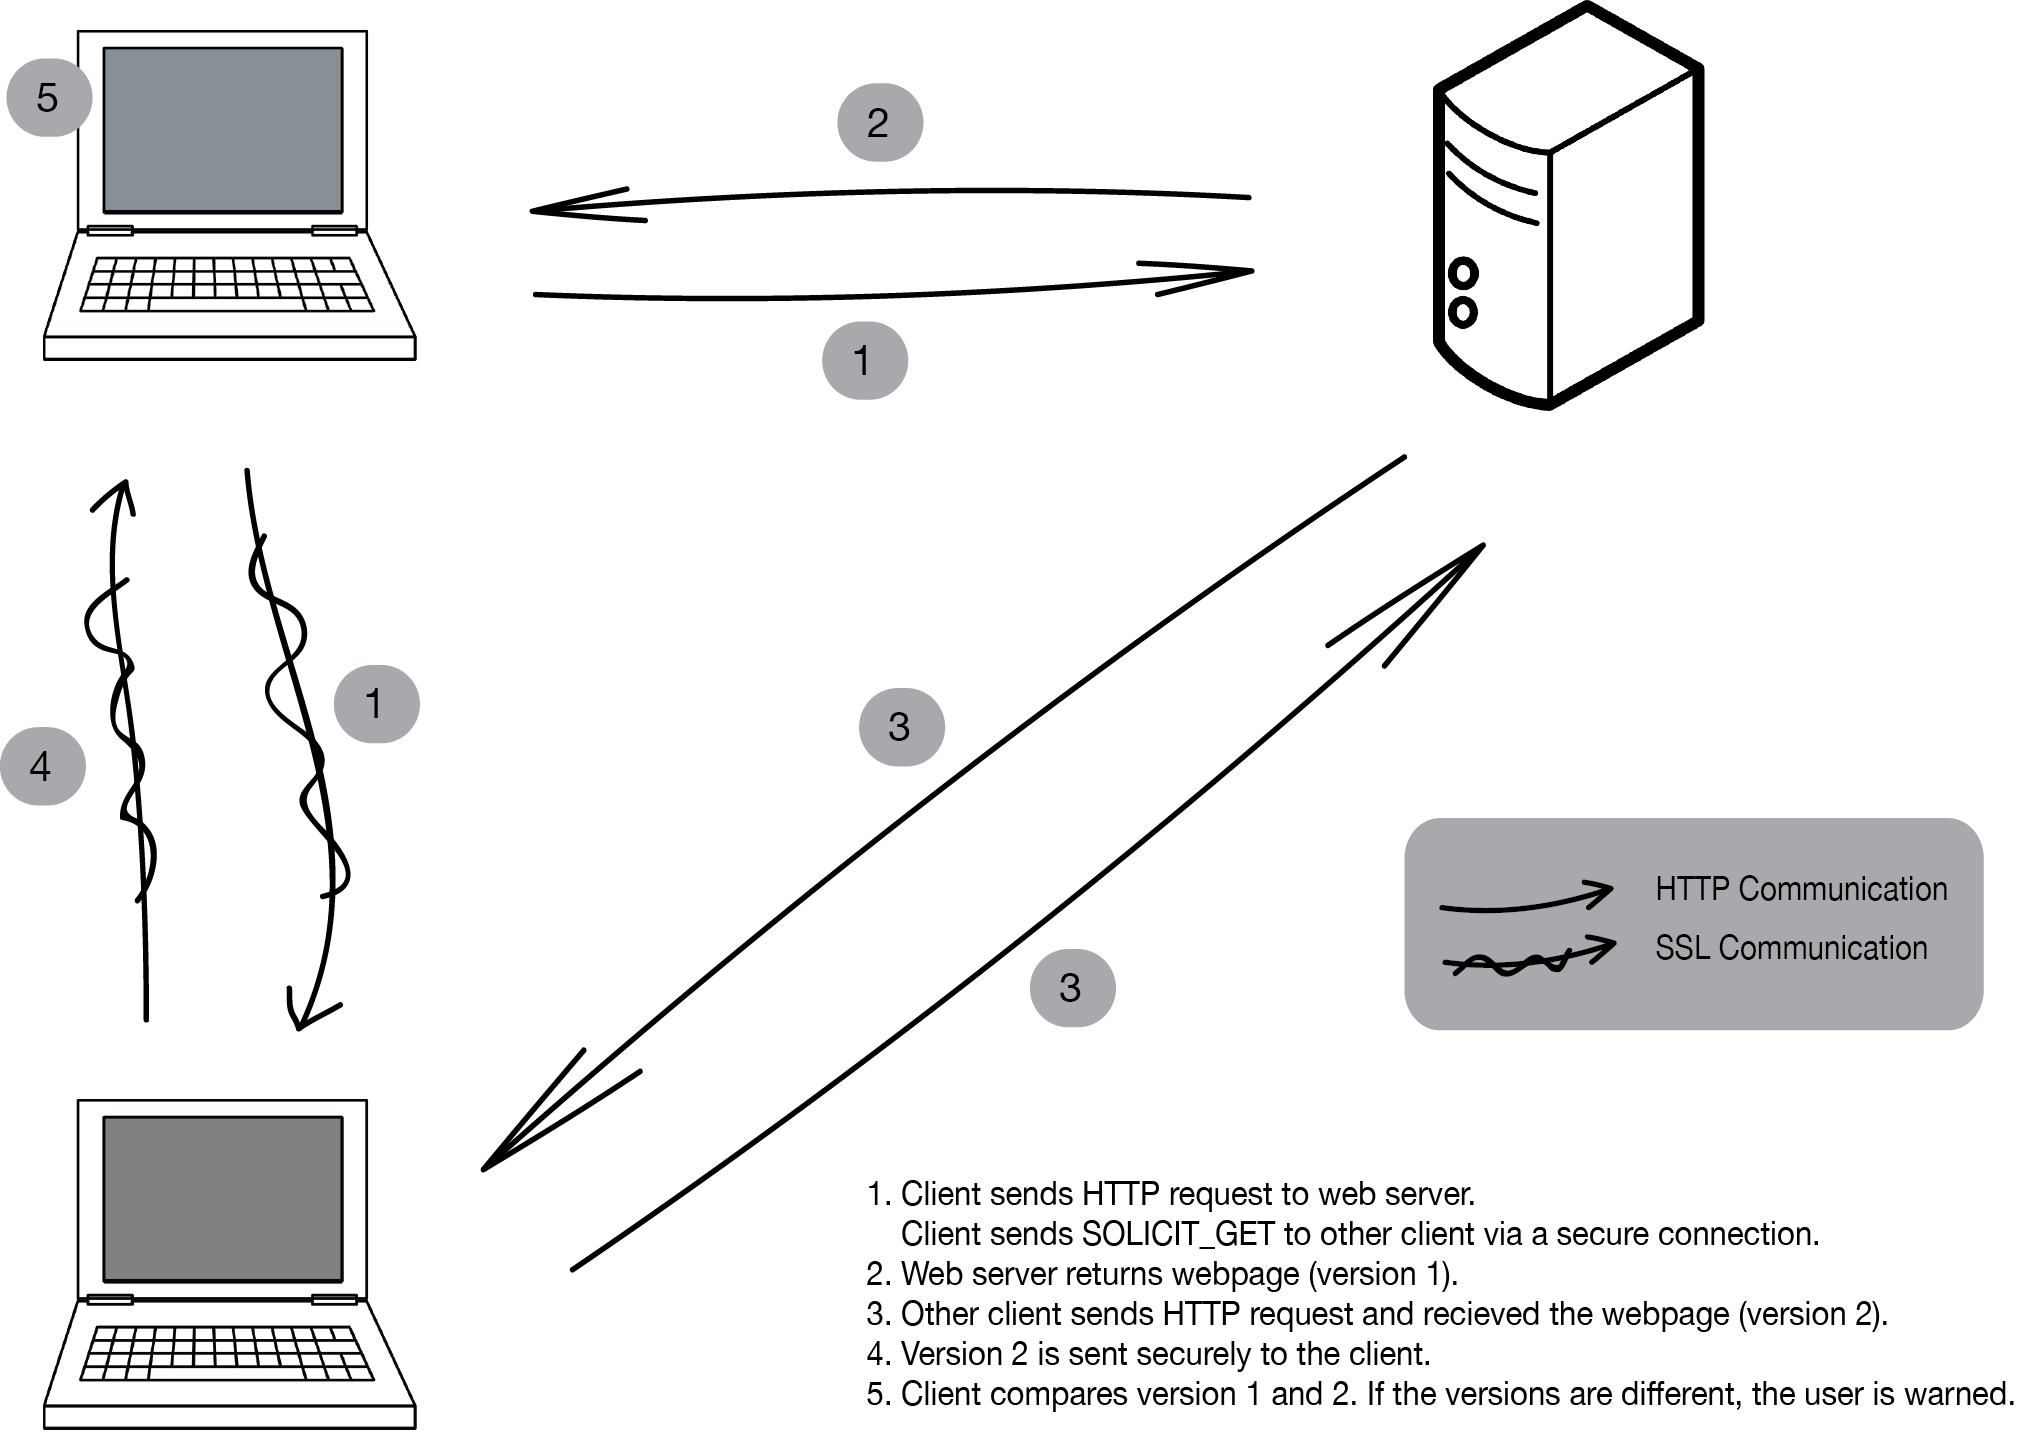
\includegraphics[scale=0.4]{./Protocol.png}
\caption{The Multisurf client-peer protocol.}
\label{fig:protocol}
\end{figure}

\subsection{Implementation}
We have implemented a working Multisurf prototype. The browser extension is implemented for the Google Chrome browser in Javascript and Python. The native client and peer applications are implemented in Python. We have made our code available on Git Hub.\footnote{\url{http://github.com/ohadf/multisurf}}
\section{Evaluation}
\label{sec:eval}

In order to evaluate Multisurf, we ask the following questions:

\begin{itemize}
\item How much does it cost to use Multisurf in terms of performance?
\item How accurately does Multisurf classify ``safe'' and ``unsafe'' sites?
\end{itemize}

We answer these questions by measuring the latency of our system, as well as analyzing the results of running our system using different comparison algorithms.

Our measurements are taken using the Alexa Top 100~\cite{alexa} websites as our dataset.  All of our experiments were performed using a laptop with a 2 GHz Intel Core 2 Duo processor.  

\subsection{Latency} 
For each web page, we measure the latency from the client; this is measuring the time for the client to make her own request, the time for the client to ask her peer to make the same request, and the time for the peer to make the request and return her response to the client.  Using the Alexa Top 50 websites, we measure the latency 50 times and take the average.  This is repeated for the four different comparison algorithms that Multisurf can use, as well as a base line measurement of the latency solely for the client to make a request.  The results are shown in Figure~\ref{fig:latency}.

\begin{figure}[htb]
\label{fig:latency}
\begin{center}
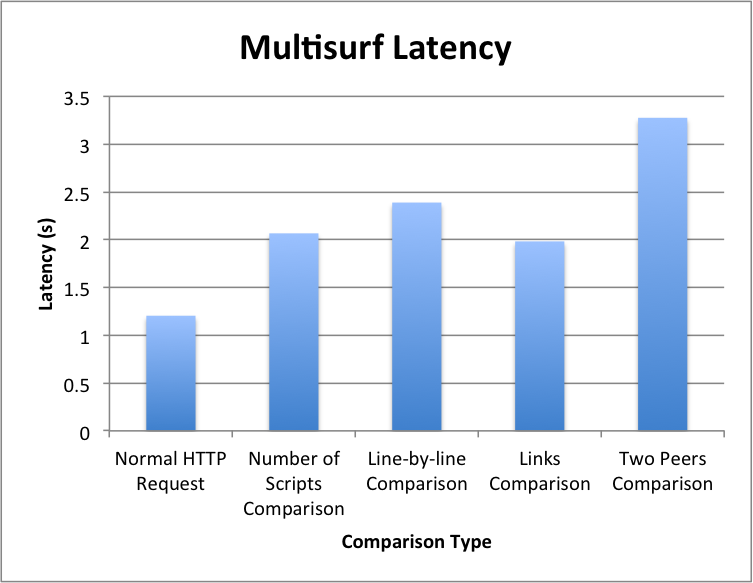
\includegraphics[width=\linewidth]{latency}
\caption{Latency of Multisurf.}
\end{center}
\end{figure}

The latency of the different methods in comparison to one another are what was expected.  When the client sends just her own request, without interacting with her peer, she has the lowest latency.  On the other hand, the highest latency occurs when the client uses two peers to determine if a site is safe; she must send her own request in addition to asking two peers to send their requests.  Overall, the latencies were relatively similar and the additional time it took to use Multisurf does not outweigh the benefits.  

\subsection{Accuracy}
We measure accuracy in terms of the number of websites that are classified as ``safe'' and ``unsafe.''  Once the client recieves her own response as well as the response her peer sends, both responses go through a comparison, and are then placed in one of six categories:

\begin{enumerate}
\item ``Safe''
\item ``Unsafe''
\item Identical responses, but no content to compare
\item Different responses, but no content to compare
\item HTTPS-Only
\item Error
\end{enumerate}

In determining accuracy, we only consider the first two categories.  A ``safe'' site is one that was determined by the comparison algorithm to not have a man in the middle attack; an ``unsafe'' site is one that was determined by the comparison algorithm to possibly have a man in the middle attack.  For our measurements, we assume that there were no man in the middle attacks and 100\% accuracy would be no ``unsafe'' sites.  We calculated the accuracy for our four different comparison methods: comparing the number of scripts, comparing line by line, comparing the links, and comparing line by line with two peers.

\subsubsection{Number of Scripts}
Figure~\ref{fig:scripts} shows the results of using Multisurf with the comparison algorithm that compares the number of scripts in each response.  The accuracy is 34.39\%.  This shows that there are a significant number of websites that send a different number of scripts in each response.

\begin{figure}[htb]
\label{fig:scripts}
\begin{center}
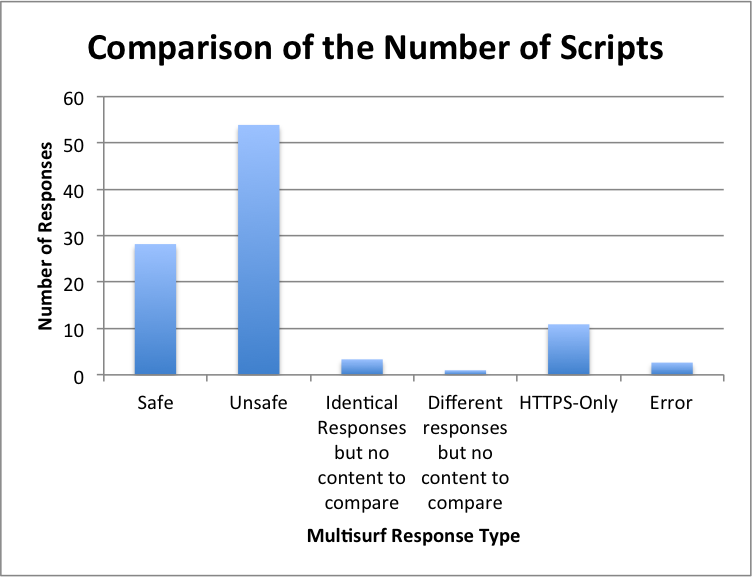
\includegraphics[width=\linewidth]{scripts}
\caption{Responses from Comparing the Number of Scripts.}
\end{center}
\end{figure}

\subsubsection{Line by Line}
When comparing the responses line by line, Multisurf exhibited only 8.72\% accuracy.  The amount of dynamic web content on the Internet is a large factor in the low accuracy rate of this method.  The results are shown in Figure~\ref{fig:lines}.

\begin{figure}[htb]
\label{fig:lines}
\begin{center}
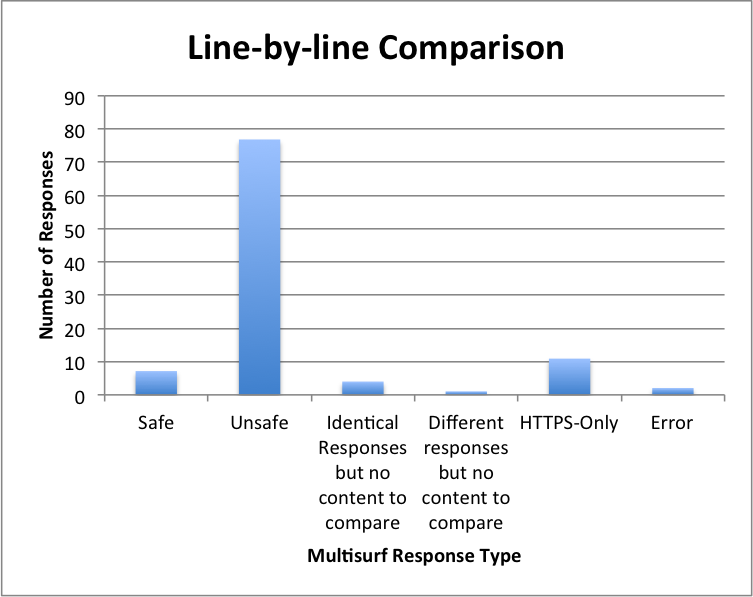
\includegraphics[width=\linewidth]{lines}
\caption{Responses from Comparing Line by Line.}
\end{center}
\end{figure}

\subsubsection{Links}
A possible man in the middle attack is to inject or change a URL in the response to take the client to a malicious site.  The Multisurf response types for comparing which links are in each response are shown in Figure~\ref{fig:links}; this method has an accuracy of 46.16\%. 

\begin{figure}[htb]
\label{fig:links}
\begin{center}
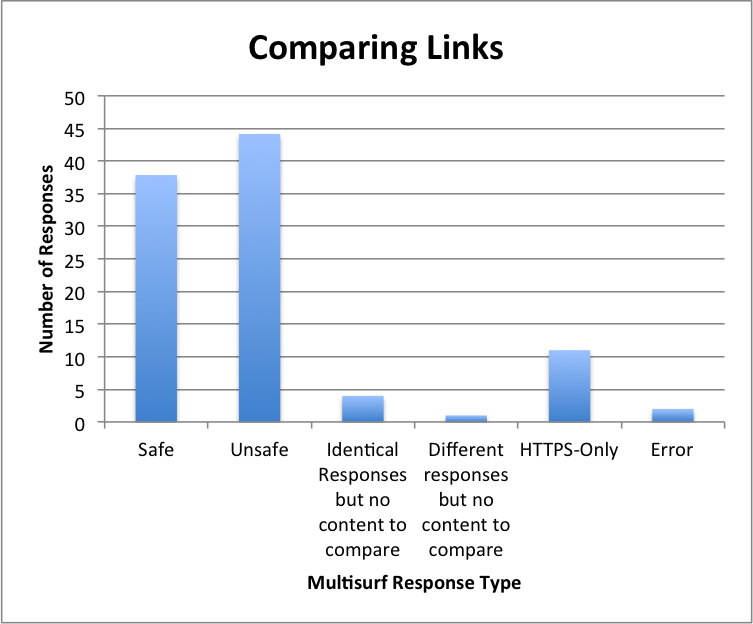
\includegraphics[width=\linewidth]{links}
\caption{Responses from Comparing Links.}
\end{center}
\end{figure}

\subsubsection{Line by Line with Two Peers}
The accuracy rates for the three comparison methods above are relatively low; this can be improved by adding a second peer.  In this case, we check to see if the response of the client is different from either of the peers' responses.  If the peers' responses are the same (as measured line by line) and the client's response is different (as measured line by line), then the site is classified as ``unsafe.''  Otherwise, the site is deemed ``safe.''  The accuracy for this method is 100\% and can be seen in Figure~\ref{fig:twopeers}.

\begin{figure}[htb]
\label{fig:peers}
\begin{center}
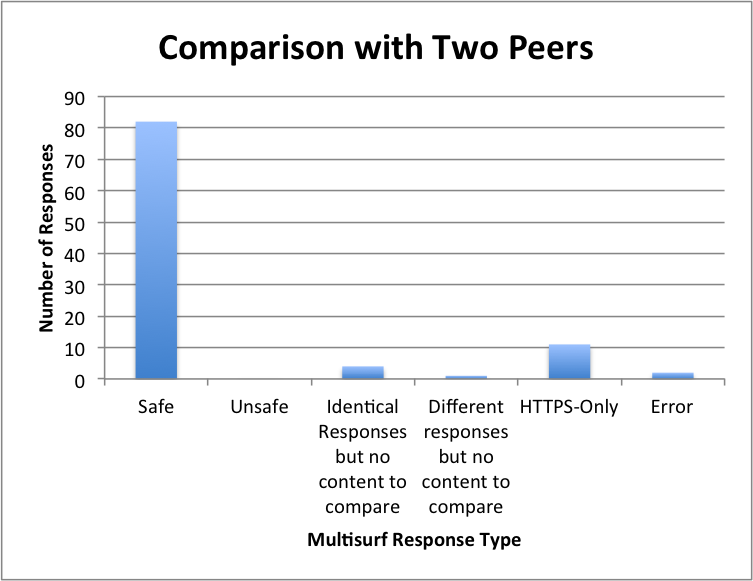
\includegraphics[width=\linewidth]{twopeers}
\caption{Responses from Comparing with Two Peers.}
\end{center}
\end{figure}

\section{Related Work}
\label{sec:related}

Related Work:

Tor: The goal of Tor is to hide the origin of a web request. However, the use of Tor is orthogonal to this work for a few reasons: (1) Tor is not suitable for every-day web browsing because it is slow and many commonly used services are not compatible with Tor, and (2) Users may not be seeking the kind of secure web browsing environment that Tor offers, i.e. they may still want to have a locale-dependent/personalized experience. Thus, our work provides the compatibility with common web services, is light-weight, and does not significantly change a user’s every-day browsing experience.

Perspectives: Rather than validating an SSL certificate by checking for certificate authority approval, with Perspectives the browser validates a certificate by checking for consistency with the certificates observed by the network notaries over time. Our system uses a similar approach to check whether web content is being served consistently across the web. Instead of having a group of trusted notary servers, the user designates a group of trusted peers/organizations that mirror the HTTP request on her behalf and relay the response they receive from the web server back to the user. The user’s browser then compares the received responses to verify that the various versions of the requested web content are consistent.            
                                                   
Web Tripwire: Using client-side javascript code, web tripwires are a way to detect many in-flight page modifications over HTTP.  Our system differs in a couple of ways: (1) We attempt to solely detect man-in-the-middle attacks, whereas web tripwires detects modifications from pop-up blockers, ad blockers, ad injectors, as well as from other sources. (2) Our system will not have access to any servers that hold web data.  Instead of comparing the requested page to a known-good representation of the requested page, we compare our requested page to a trusted peer/organization’s request of the same page.  

Mitigating Man in the Middle Attack over Secure Sockets Layer: This paper presents and implements a novel approach to solve man-in-the-middle attacks over SSL.  There has been related work, such as this, on the topic of MITM attacks over SSL, but few that cover these attacks simply over HTTP.  Our system differs by detecting attacks using trusted peers/organizations, as opposed to solving them using cryptographic functionality.

\section{Future Work}
\label{sec:future}

Example of incorporation citations~\cite{coral:nsdi04}.

-More fine-grained comparison algorithms (handle more dynamic content, more accuracy)
-More user-friendly display in browser
-Methods to not rely on a peer always being available
-Optimizations (concurrent peer interaction as opposed to consecutive)
-Learning algorithm


\section{Conclusions}
\label{sec:conclusion}



%% Bibliography
%\vspace{-1ex}
%\linespread{1.0}
%\setlength{\bibsep}{1pt}
%\footnotesize
\small
\bibliography{local}
\bibliographystyle{abbrvnat}

\end{document}

